\subsection{Results}\label{Testing:Results}
	In this section we will go over the results for each of the test cases in the preceding section. We will compare the results with each other and also compare most of the cases to the "No throttle mediator" scenario.
	
	\begin{shaded}
	To see all the results of our tests in their raw forms, we refer you to appendix \ref{RawResults}.
	\end{shaded}
	 
    \textbf{Test case 1:}\\
    In test 1 we wanted to find out how the ESB would perform with a low timeout. From our expectations we want to see that the average time for messages to arrive is low, but we do not expect this test to have as good a percentage as the rest. 
    
	\begin{figure}[H]
		\centering
		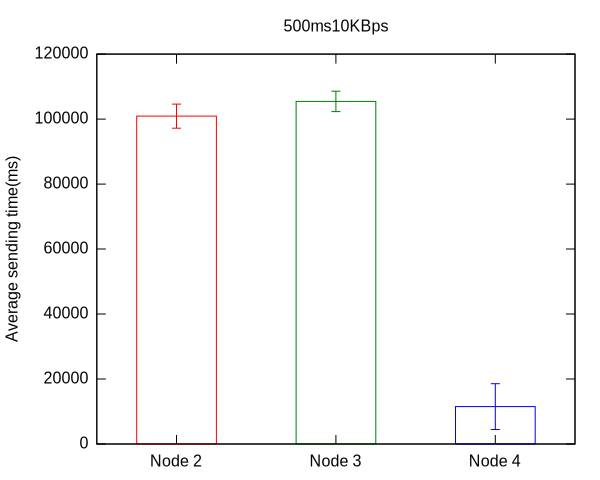
\includegraphics[scale=0.5]{500ms10KBps_time}
		\caption{Time graph, timeout equal to 500 and bandwidth of 10kBps} 
		\label{figure:results:500ms10KBps_time}
	\end{figure}
	
	\begin{figure}[H]
		\centering
		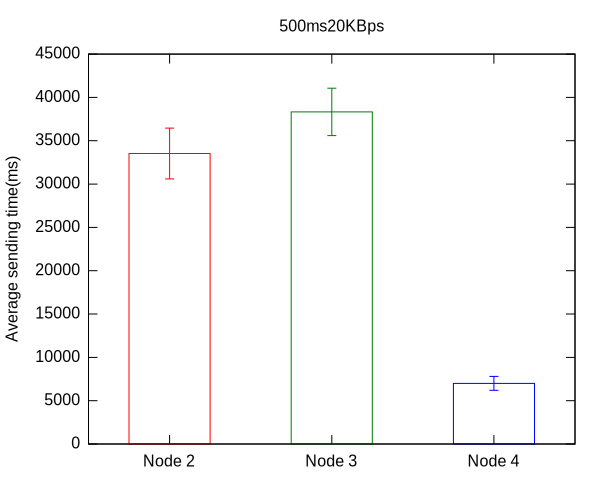
\includegraphics[scale=0.5]{500ms20KBps_time}
		\caption{Time graph, timeout equal to 500 and bandwidth of 20kBps} 
		\label{figure:results:500ms20KBps_time}
	\end{figure}
    
    The actual results do indeed match our expectation quite well. As you can see in figure \ref{figure:results:500ms20KBps_time} the time taken is quite low, if we compare that time to the time in figure \ref{figure:results:2000ms20KBps_time} we can easily see that the lower timeout has an effect on the results and in most of the cases it is correct that the lower timeout does make the ESB quicker.
    
    \begin{figure}[H]
		\centering
		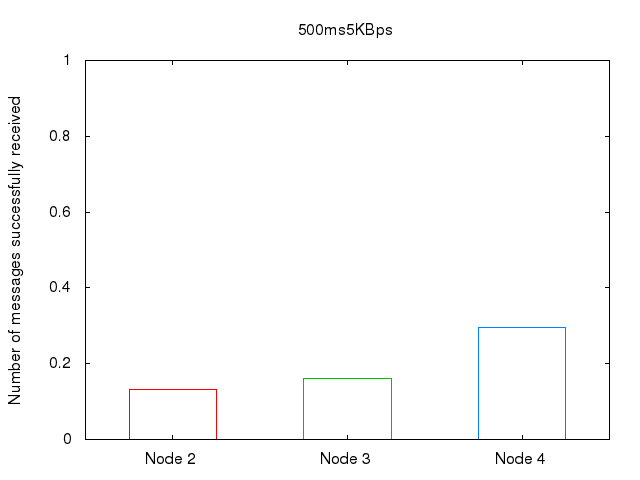
\includegraphics[scale=0.5]{500ms5KBps_messages}
		\caption{Message graph, timeout equal to 500 and bandwidth of 5kBps} 
		\label{figure:results:500ms5KBps_messages}
	\end{figure}
    
    \textbf{Test case 2:}\\
    
    \begin{figure}[H]
		\centering
		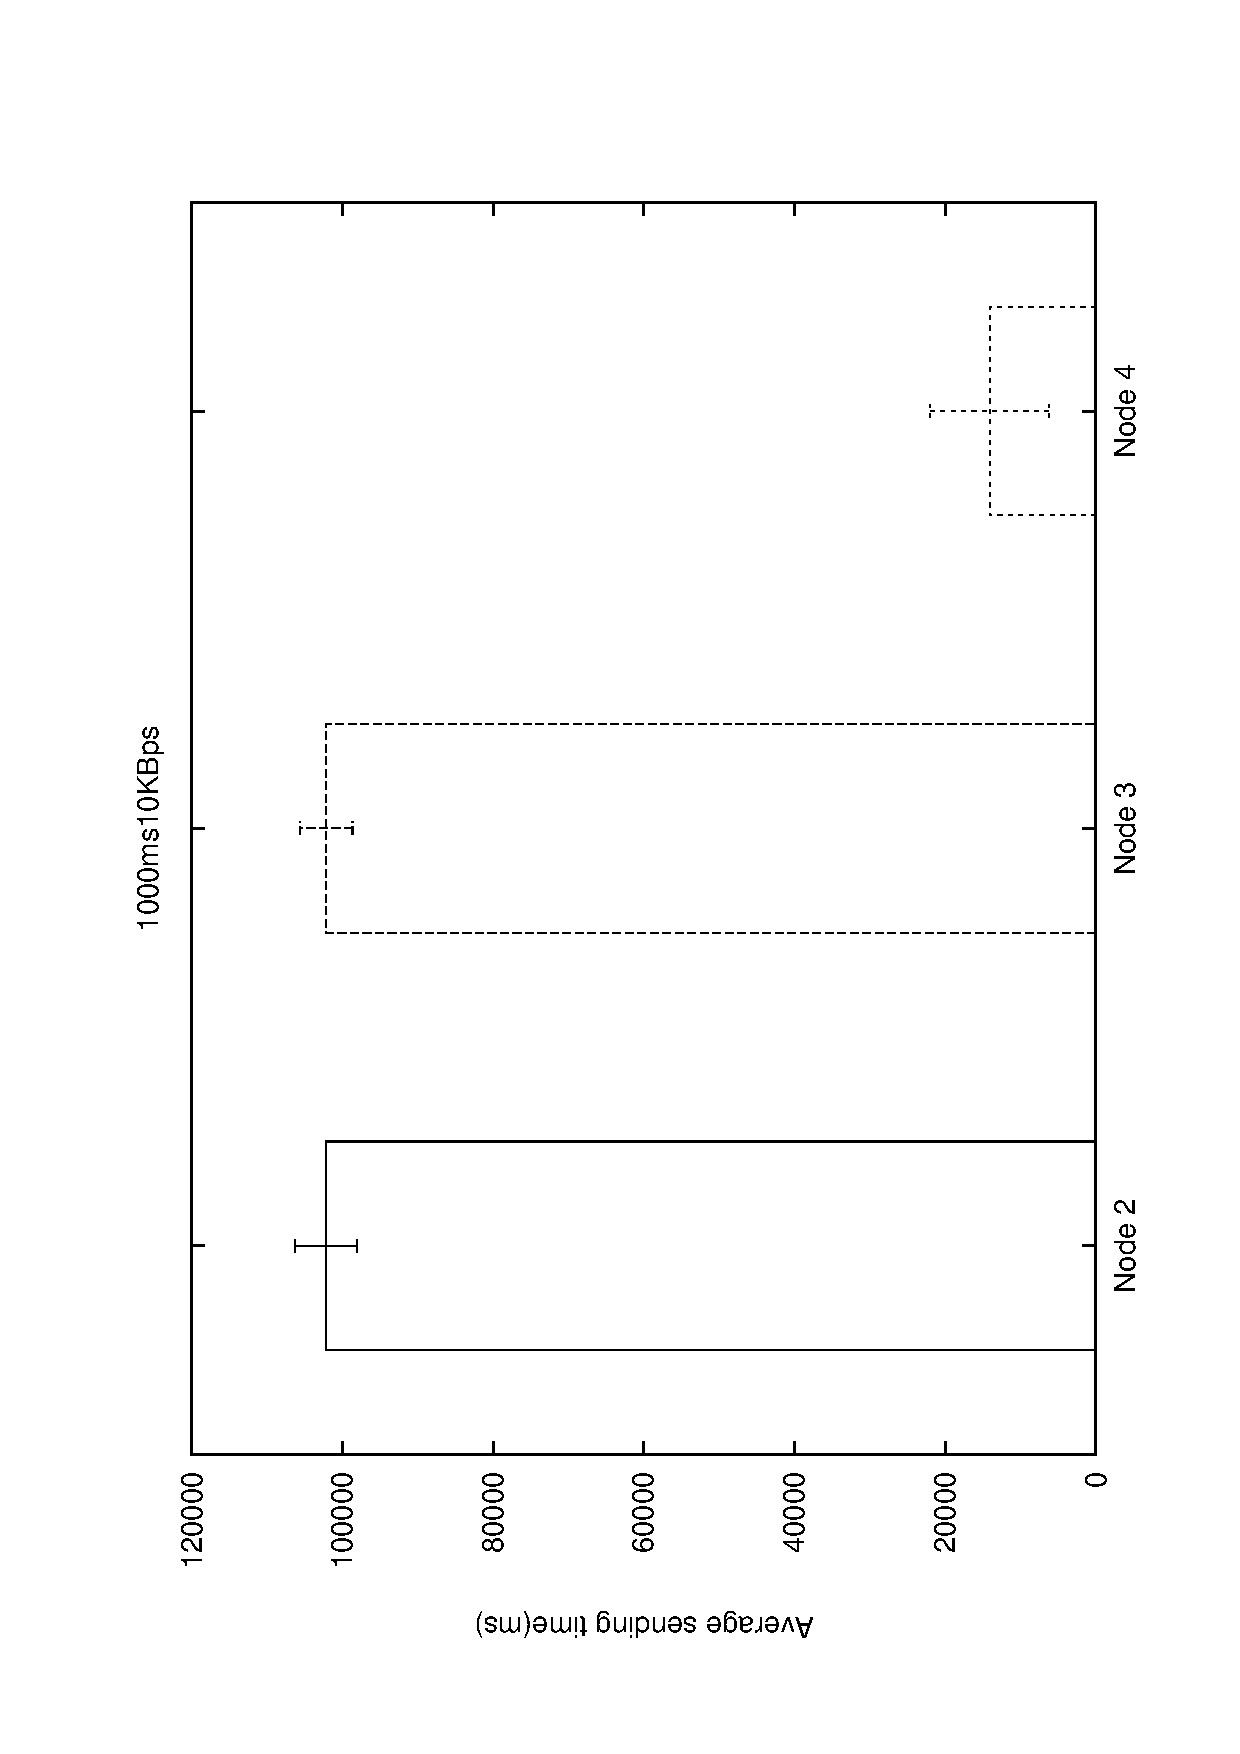
\includegraphics[scale=0.5]{1000ms10KBps_time}
		\caption{Time graph, timeout equal to 1000 and bandwidth of 10kBps} 
		\label{figure:results:1000ms10KBps_time}
	\end{figure}
	
	\begin{figure}[H]
		\centering
		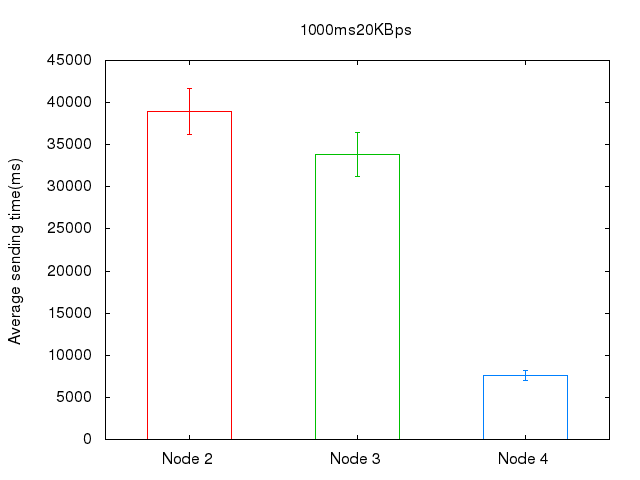
\includegraphics[scale=0.5]{1000ms20KBps_time}
		\caption{Time graph, timeout equal to 1000 and bandwidth of 20kBps} 
		\label{figure:results:1000ms20KBps_time}
	\end{figure}
	
	\begin{figure}[H]
		\centering
		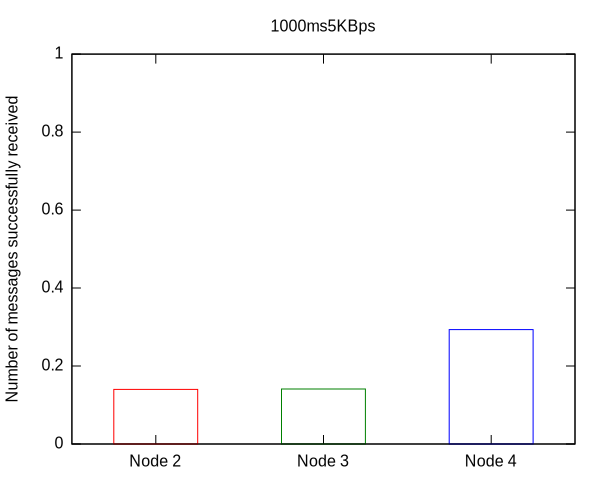
\includegraphics[scale=0.5]{1000ms5KBps_messages}
		\caption{Message graph, timeout equal to 1000 and bandwidth of 5kBps} 
		\label{figure:results:1000ms5KBps_messages}
	\end{figure}
    
    \textbf{Test case 3:}\\
    
    \begin{figure}[H]
		\centering
		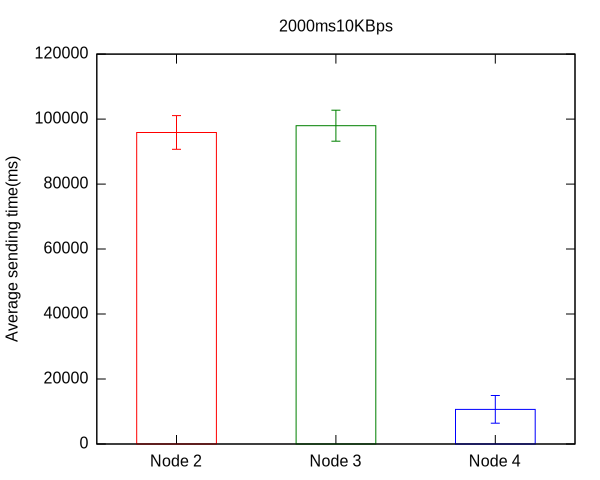
\includegraphics[scale=0.5]{2000ms10KBps_time}
		\caption{Time graph, timeout equal to 2000 and bandwidth of 10kBps} 
		\label{figure:results:2000ms10KBps_time}
	\end{figure}
	
	\begin{figure}[H]
		\centering
		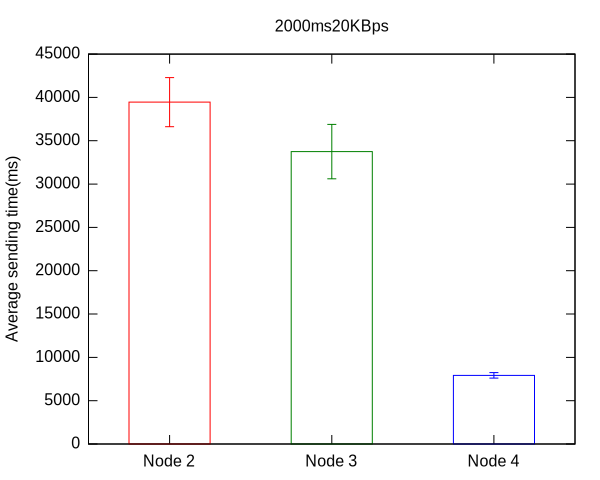
\includegraphics[scale=0.5]{2000ms20KBps_time}
		\caption{Time graph, timeout equal to 2000 and bandwidth of 20kBps} 
		\label{figure:results:2000ms20KBps_time}
	\end{figure}
	
	\begin{figure}[H]
		\centering
		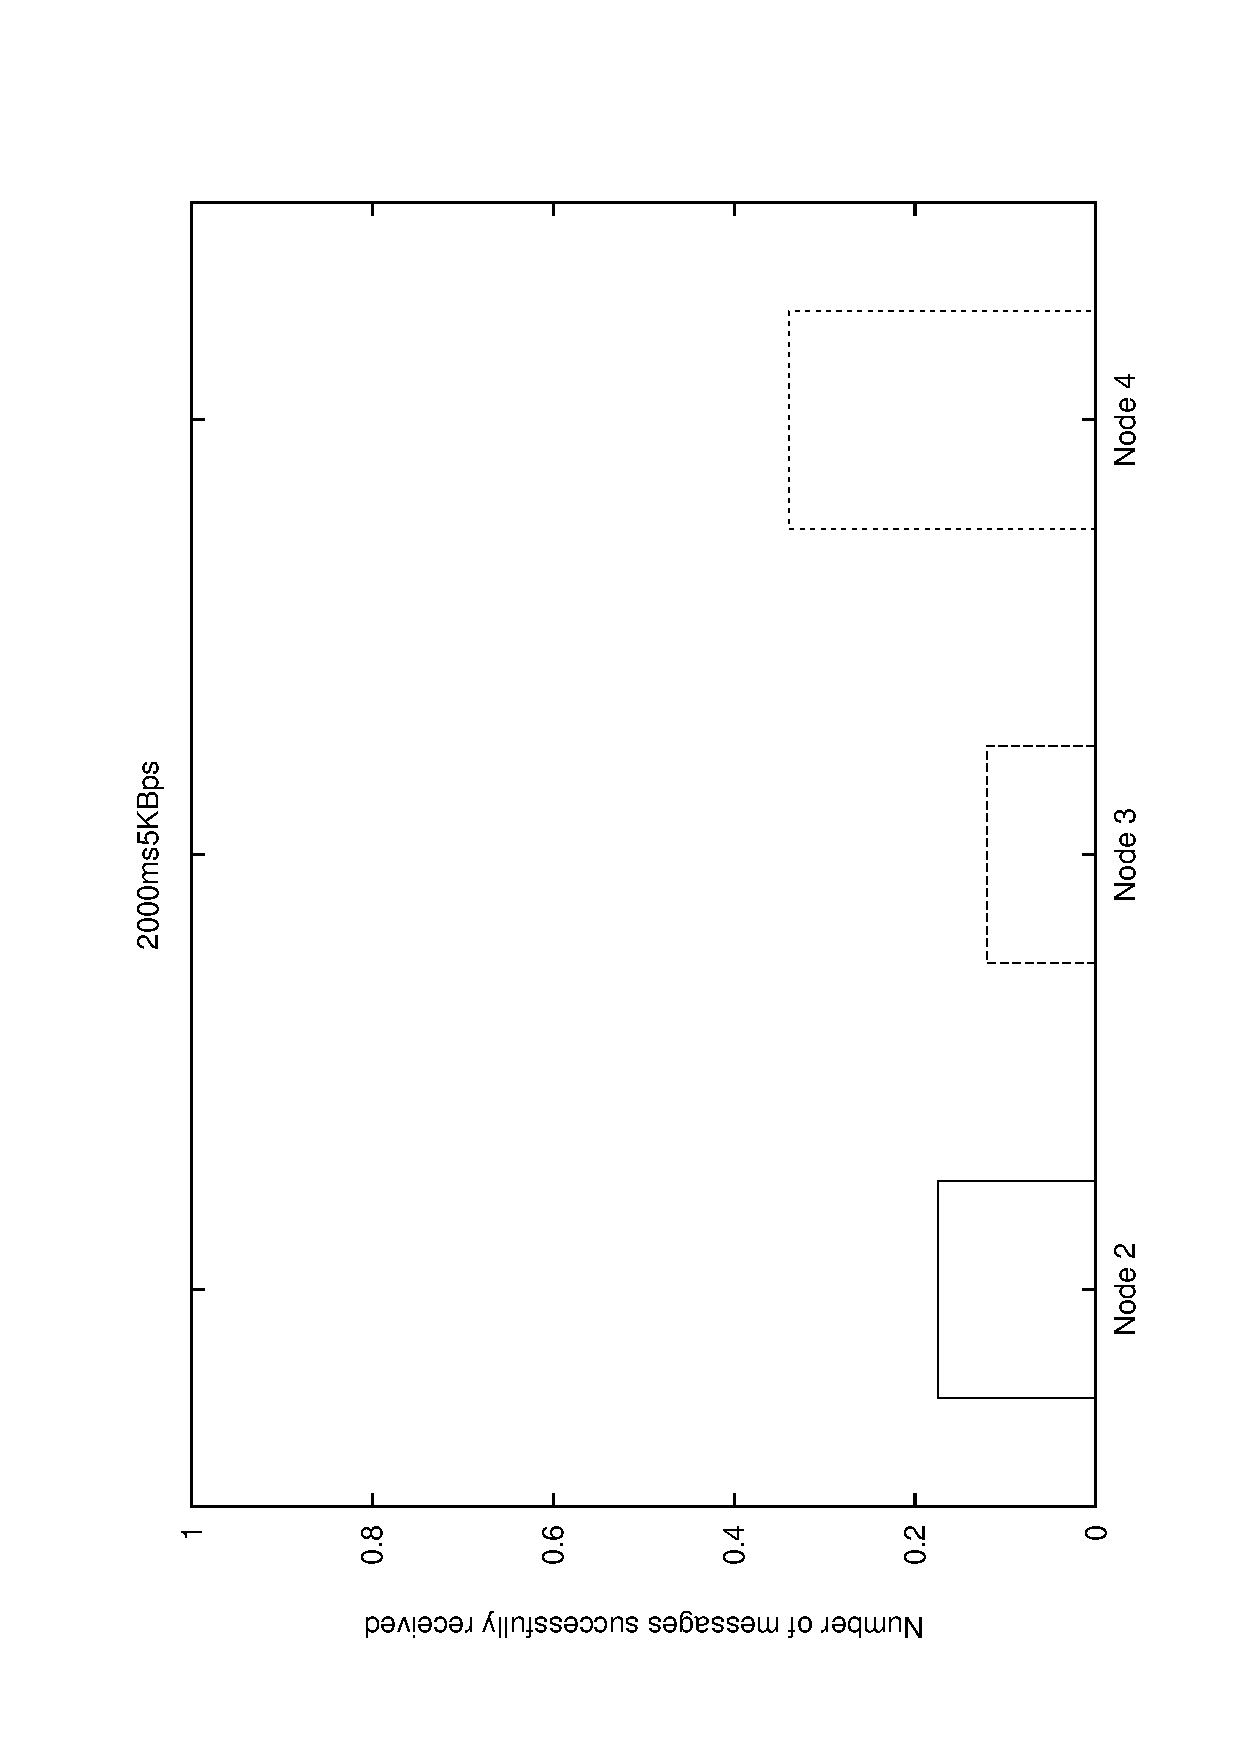
\includegraphics[scale=0.5]{2000ms5KBps_messages}
		\caption{Message graph, timeout equal to 2000 and bandwidth of 5kBps} 
		\label{figure:results:2000ms5KBps_messages}
	\end{figure}
    
    \textbf{Test case 4:}\\
    
    \begin{figure}[H]
		\centering
		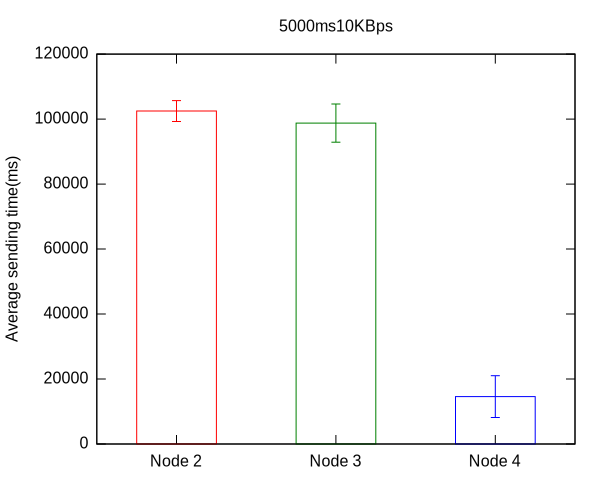
\includegraphics[scale=0.5]{5000ms10KBps_time}
		\caption{Time graph, timeout equal to 5000 and bandwidth of 10kBps} 
		\label{figure:results:5000ms10KBps_time}
	\end{figure}
	
	\begin{figure}[H]
		\centering
		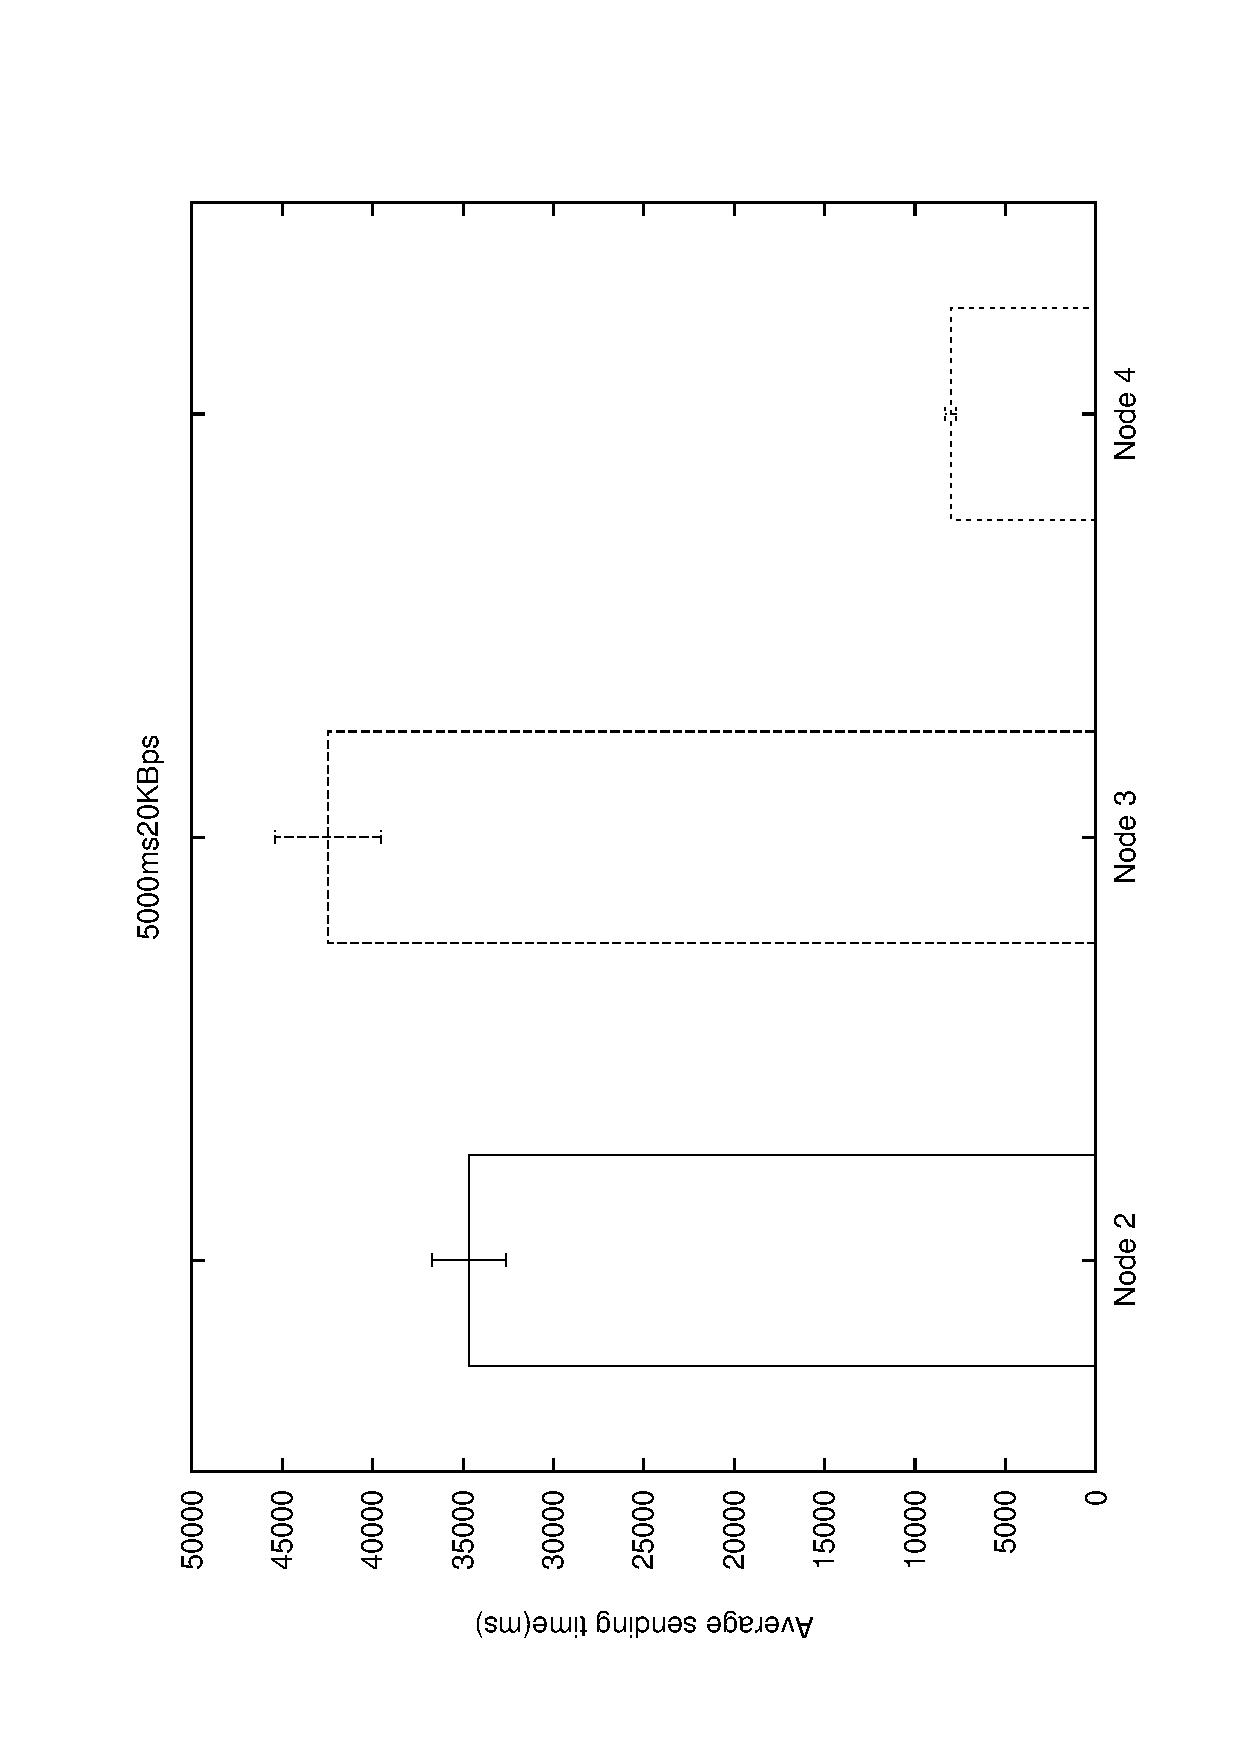
\includegraphics[scale=0.5]{5000ms20KBps_time}
		\caption{Time graph, timeout equal to 5000 and bandwidth of 20kBps} 
		\label{figure:results:5000ms20KBps_time}
	\end{figure}
	
	\begin{figure}[H]
		\centering
		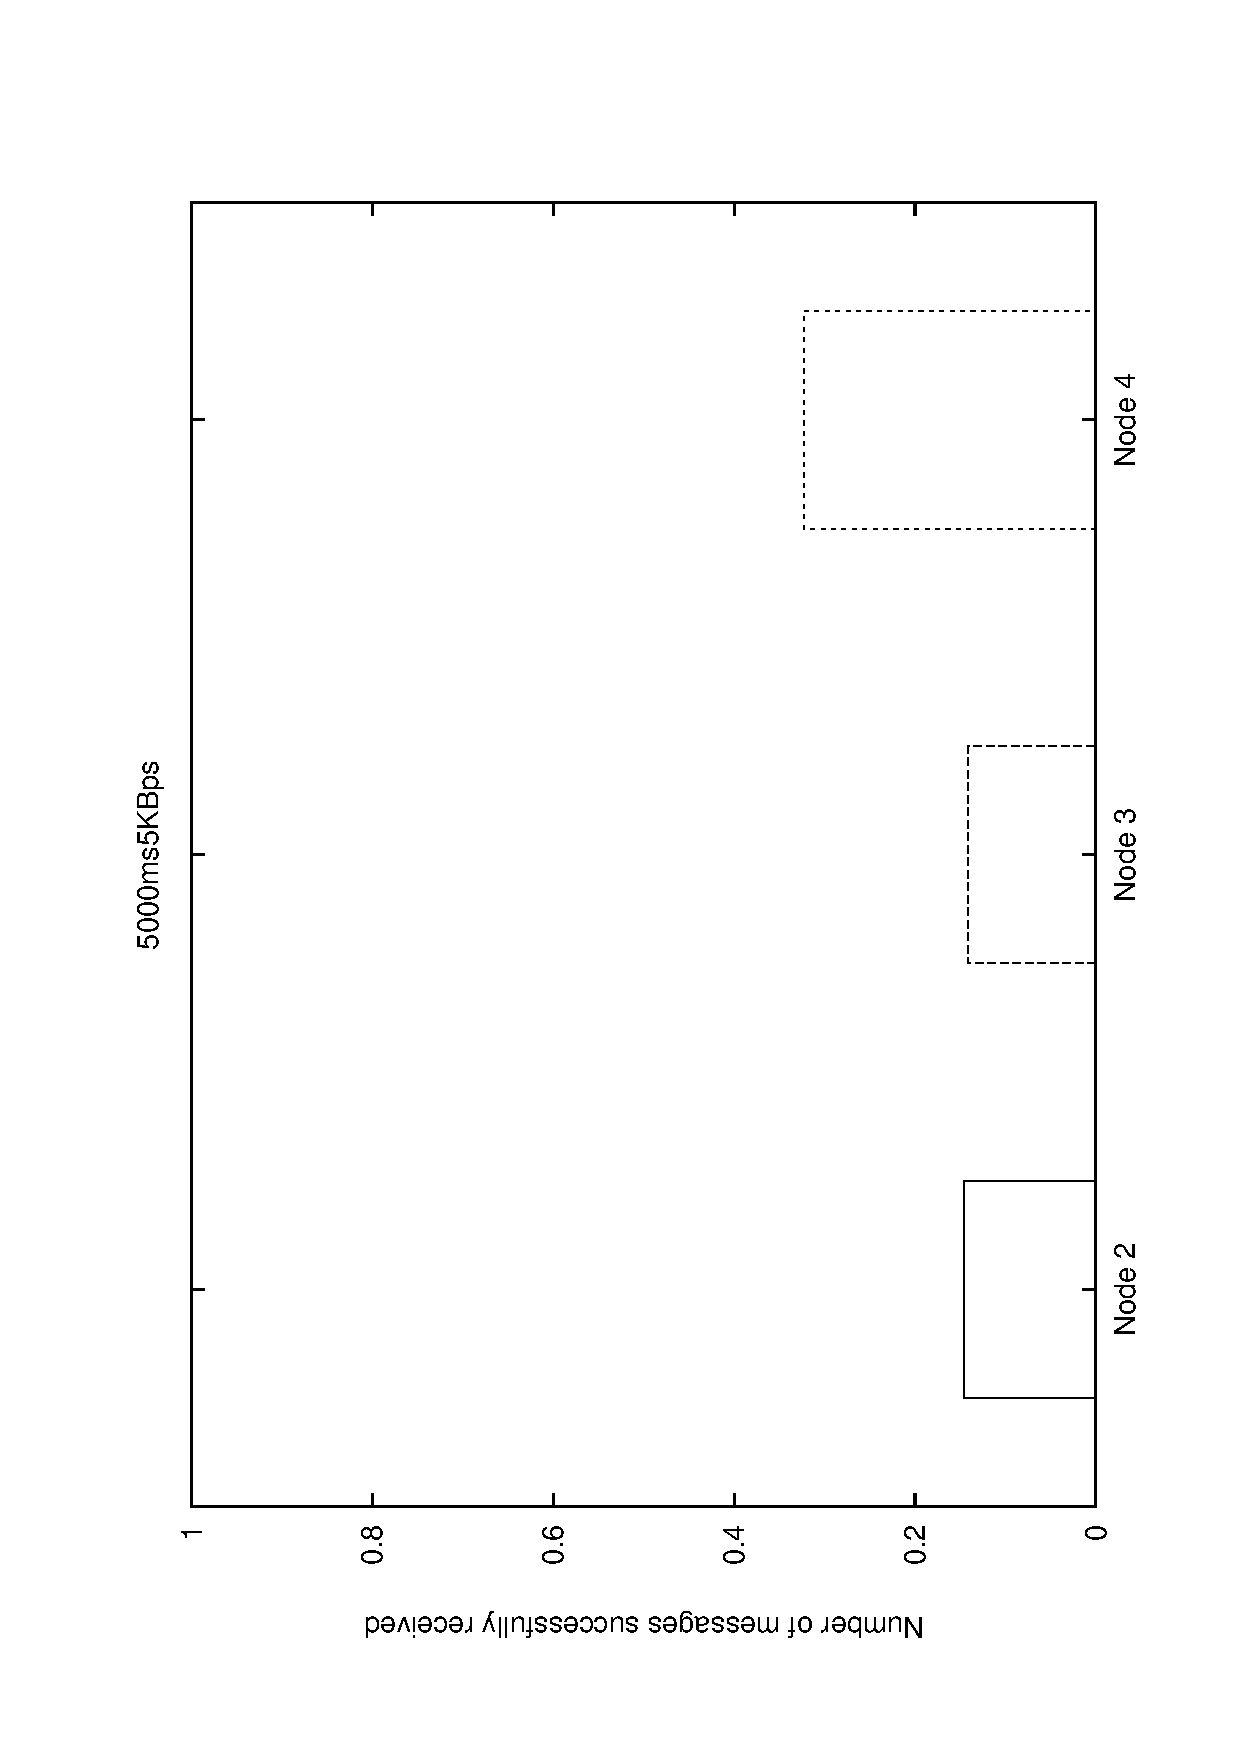
\includegraphics[scale=0.5]{5000ms5KBps_messages}
		\caption{Message graph, timeout equal to 5000 and bandwidth of 5kBps} 
		\label{figure:results:5000ms5KBps_messages}
	\end{figure}
    
    \textbf{Test case 5:}\\
    
    \begin{figure}[H]
		\centering
		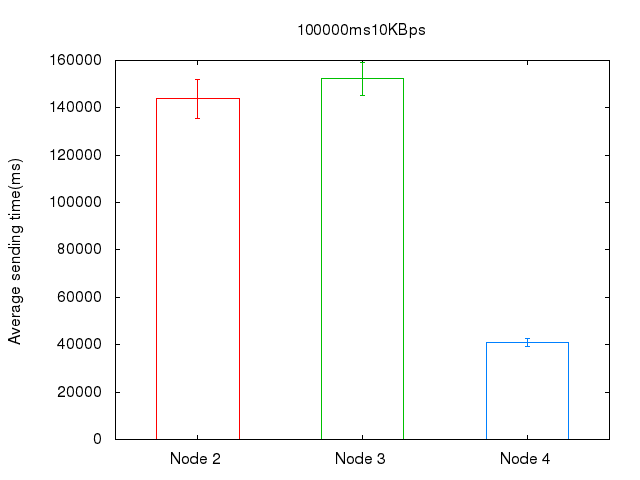
\includegraphics[scale=0.5]{100000ms10KBps_time}
		\caption{Time graph, timeout equal to 100000 and bandwidth of 10kBps} 
		\label{figure:results:100000ms10KBps_time}
	\end{figure}
	
	\begin{figure}[H]
		\centering
		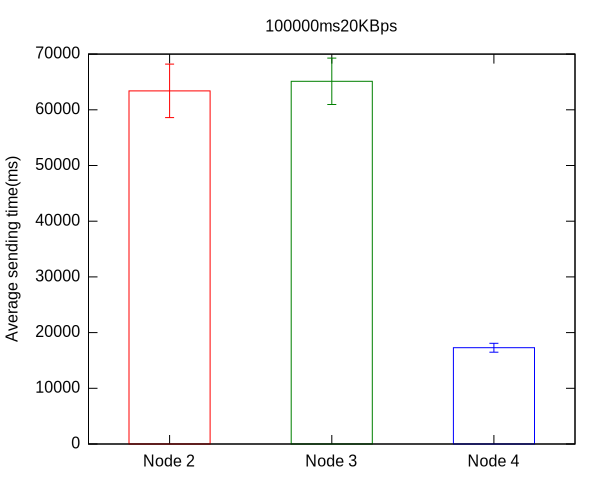
\includegraphics[scale=0.5]{100000ms20KBps_time}
		\caption{Time graph, timeout equal to 100000 and bandwidth of 20kBps} 
		\label{figure:results:100000ms20KBps_time}
	\end{figure}
	
	\begin{figure}[H]
		\centering
		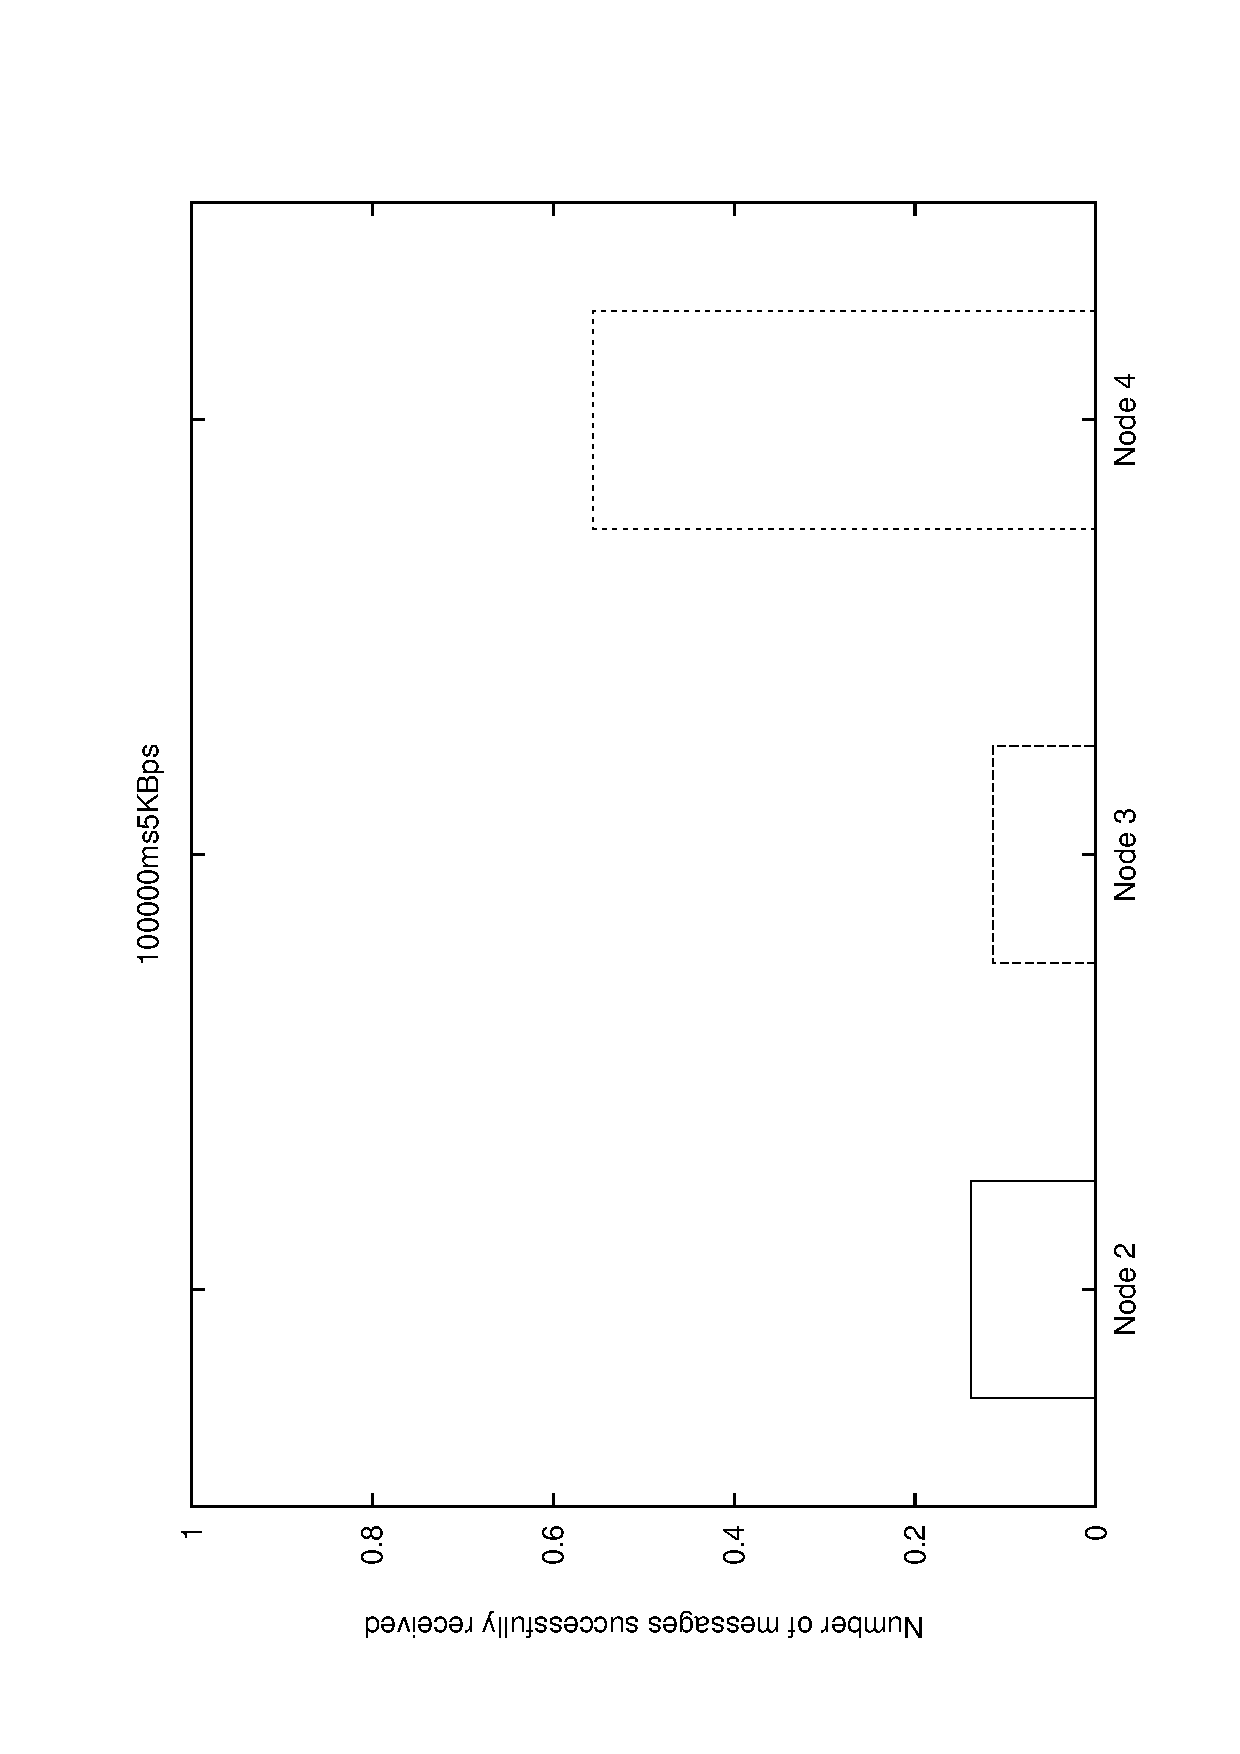
\includegraphics[scale=0.5]{100000ms5KBps_messages}
		\caption{Message graph, timeout equal to 100000 and bandwidth of 5kBps} 
		\label{figure:results:100000ms5KBps_messages}
	\end{figure}
    
    \textbf{Test case 6:}\\
    
    \begin{figure}[H]
		\centering
		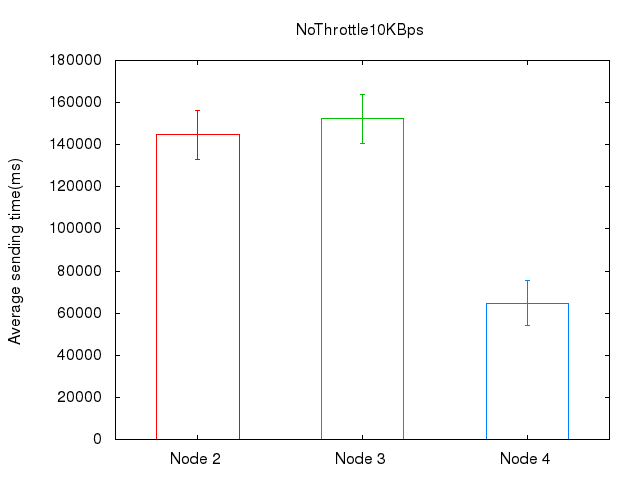
\includegraphics[scale=0.5]{NoThrottle10KBps_time}
		\caption{Time graph, no throttle mediator and bandwidth of 10kBps} 
		\label{figure:results:NoThrottle10KBps_time}
	\end{figure}
	
	\begin{figure}[H]
		\centering
		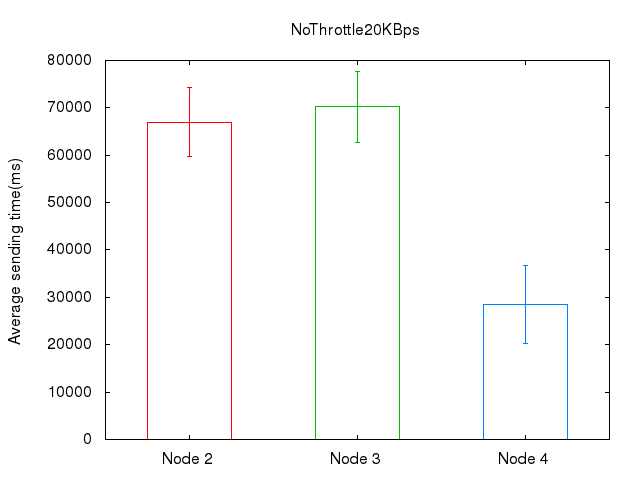
\includegraphics[scale=0.5]{NoThrottle20KBps_time}
		\caption{Time graph, no throttle mediator and bandwidth of 20kBps} 
		\label{figure:results:NoThrottle20KBps_time}
	\end{figure}
	
	\begin{figure}[H]
		\centering
		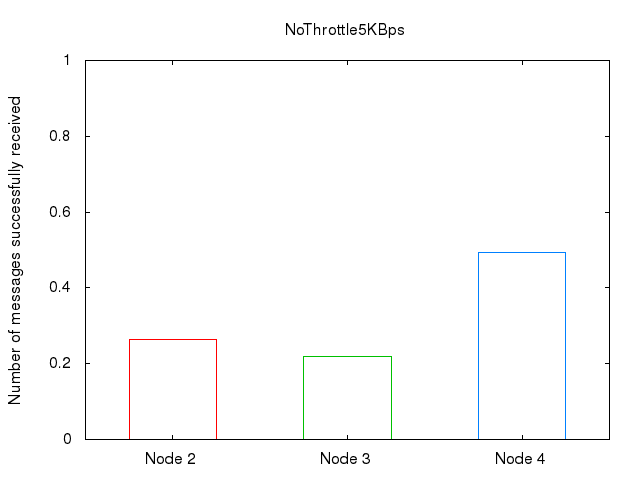
\includegraphics[scale=0.5]{NoThrottle5KBps_messages}
		\caption{Time graph, no throttle mediator and bandwidth of 5kBps} 
		\label{figure:results:NoThrottle5KBps_messages}
	\end{figure}
